\documentclass{report}
\usepackage[spanish]{babel}
\usepackage[utf8]{inputenc}
\usepackage{graphicx, longtable, float, titlesec, hyperref, enumitem, dingbat, soul, multicol, listings}
\usepackage[dvipsnames]{xcolor}
\usepackage[margin=2cm]{geometry}

% Cambia el color de los links
\hypersetup{hidelinks}

% Generamos un comando para saltar pagina con las secciones
\NewDocumentCommand{\cpsection}{s o m}{%
  \clearpage
  \IfBooleanTF{#1}
    {\section*{#3}}
    {%
      \IfNoValueTF{#2}
        {\section{#3}}
        {\section[#2]{#3}}%
    }%
}

% Python Code
\lstdefinestyle{Python}{
  commentstyle=\color{brown},
  keywordstyle=\color{violet},
  numberstyle=\tiny\color{gray},
  stringstyle=\color{purple},
  basicstyle=\ttfamily\footnotesize,
  breakatwhitespace=false,         
  breaklines=true,                 
  captionpos=b,                    
  keepspaces=true,                 
  numbers=left,                    
  numbersep=5pt,                  
  showspaces=false,                
  showstringspaces=false,
  showtabs=false,                  
  tabsize=2,
  literate={ñ}{{\~n}}1 {á}{{\'a}}1 {é}{{\'e}}1 {í}{{\'i}}1 {ó}{{\'o}}1 {ú}{{\'u}}1
}
\lstset{style=Python}

% Elimina la palabra "Capítulo" de los títulos de los capítulos
\titleformat{\chapter}[display]
  {\normalfont\bfseries}{}{0pt}{\Huge\thechapter.\space}

\titleformat{name=\chapter,numberless}[display]
  {\normalfont\bfseries}{}{0pt}{\Huge}

\titlespacing*{\chapter}{0pt}{-50pt}{20pt}

% Personalización del índice de listados
\renewcommand{\lstlistingname}{Código}  % Cambiar el nombre de "Listing" a "Código"
\renewcommand{\lstlistlistingname}{Índice de Códigos}

% Añade numeración a los subsubsection*s y los añade al índice
\setcounter{secnumdepth}{4}
\setcounter{tocdepth}{4}

\begin{document}
  \begin{titlepage}
      \centering
      
\includegraphics[width=0.6\textwidth]{./.img/logo.jpg}\\
      \vspace{1cm}
      \LARGE Técnicas de Inteligencia Artificial\\
      \vspace{0.5cm}
      \Large Ingeniería Informática de Gestión y Sistemas de Información\\
      \vspace{3cm}
      \Huge Practica 4\\
      \huge Reinforcement Learning\\
      \vspace{2.5cm}
      \Large Autor(es):\\
      \vspace{0.2cm}
      \large Xabier Gabiña\\
      \large Diego Montoya\\
      \vfill
      \today
  \end{titlepage}
  \tableofcontents
  \listoffigures
  %\listoftables
  \lstlistoflistings 
  \chapter{Introducción} % * TERMINADO
    \paragraph*{}{
      En este proyecto de la asignatura de Técnicas de inteligencia artificial implementaremos iteración de valor y Q-learning; primero realizaremos un agente off-line de iteración de valores, pe lo que buscamos es implementar un agente inteligente basado en el modelo de Q-learning en el cual implementaremos el aprendizaje por refuerzo para nuestro Pacman. El objetivo es lograr que nuestro agente sea capaz de tomar decisiones mediante la obtención de recompensas basadas en las acciones que elija. Para lograr esto la practica nos llevará por 6 aspectos clave del aprendizaje por refuerzo.

      \begin{itemize}
        \item \textbf{Implementación básica de Q-learning:} Se comenzará con la creación de un agente que utiliza el algoritmo de Q-learning para aprender de sus interacciones con el entorno. Este agente actualizará sus valores de acción (Q-values) en función de las recompensas recibidas y las transiciones entre estados.
        \item \textbf{Selección de acciones con Epsilon-Greedy:} Para mejorar la exploración del entorno y evitar quedar atrapado en una política subóptima, se implementará una estrategia epsilon-greedy, donde el agente explorará acciones aleatorias en una fracción del tiempo.
        \item \textbf{Aplicación de Q-learning en Gridworld:} Inicialmente, el agente se entrenará en un entorno sencillo, conocido como Gridworld, para aprender a maximizar sus recompensas. A medida que el agente interactúa con el entorno, ajustará su política de manera iterativa.
        \item \textbf{Mejora de la política para Pacman:} Una vez que el agente ha aprendido en entornos más sencillos, se aplicará el algoritmo de Q-learning en el juego de Pacman, primero en un entorno pequeño (smallGrid), luego en entornos más complejos (mediumGrid). Durante esta fase, se evaluará la capacidad del agente para aprender y explotar su política en un entorno más desafiante.
      \end{itemize}

      Al finalizar esta practica tendremos un agente Pacman con la capacidad de aprender y así aplicar una estrategia óptima para maximizar su rendimiento en diferentes mapas.
    }
  \chapter{Ejercicios} % * TERMINADO
    \section{Iteración de valores} % * TERMINADO
      \subsection*{Descripción}
        \paragraph*{}{
          El primer ejercicio se trata de implementar un agente que realice la iteración de valores. 
          Un agente de Iteración de Valores toma un proceso de decisión de Markov en la inicialización y ejecuta la iteración de valores durante un número dado de iteraciones utilizando el factor de descuento proporcionado.
        }
      \subsection*{Implementación}
\begin{lstlisting}[language=Python, caption=Iteración de valores]
class ValueIterationAgent(ValueEstimationAgent):
    """
        * Please read learningAgents.py before reading this.*

        A ValueIterationAgent takes a Markov decision process
        (see mdp.py) on initialization and runs value iteration
        for a given number of iterations using the supplied
        discount factor.
    """
    def __init__(self, mdp, discount = 0.9, iterations = 100):
        """
          Your value iteration agent should take an mdp on
          construction, run the indicated number of iterations
          and then act according to the resulting policy.

          Some useful mdp methods you will use:
              mdp.getStates()
              mdp.getPossibleActions(state)
              mdp.getTransitionStatesAndProbs(state, action)
              mdp.getReward(state, action, nextState)
              mdp.isTerminal(state)
        """
        self.mdp = mdp
        self.discount = discount
        self.iterations = iterations
        self.values = util.Counter() # A Counter is a dict with default 0
        self.runValueIteration()

    def runValueIteration(self):
        # Write value iteration code here
        for _ in range(self.iterations):
            new_values = self.values.copy()
            for state in self.mdp.getStates():
                if not self.mdp.isTerminal(state):
                    new_values[state] = max(self.computeQValueFromValues(state, action) for action in self.mdp.getPossibleActions(state))
            self.values = new_values


    def getValue(self, state):
        """
          Return the value of the state (computed in __init__).
        """
        return self.values[state]


    def computeQValueFromValues(self, state, action):
        """
        computeQValueFromValues(state, action) devuelve el valor Q del par (estado, acción)
        dado por la función de valor dada por self.values. Nota: Recuerda que para calcular
        el valor de un estado calcularemos los q_values (estado,acción), es decir los valores
        de las acciones posibles para quedarnos con el mayor (max de entre los q_values).
        """
        q_value = 0
        for next_state, prob in self.mdp.getTransitionStatesAndProbs(state, action):
            q_value += prob * (self.mdp.getReward(state, action, next_state) + self.discount * self.values[next_state])
        return q_value
        

    def computeActionFromValues(self, state):
        """
        computeActionFromValues(state) calcula la mejor acción de acuerdo con la función de
        valor dada por self.values. Es decir, de acuerdo al estado siguiente al que nos lleva
        cada acción y que mayor valor tiene. Este método llamará al siguiente.
        """
        if self.mdp.isTerminal(state):
            return None

        return max(self.mdp.getPossibleActions(state), key=lambda x: self.computeQValueFromValues(state, x))
        

    def getPolicy(self, state):
        return self.computeActionFromValues(state)

    def getAction(self, state):
        "Returns the policy at the state (no exploration)."
        return self.computeActionFromValues(state)

    def getQValue(self, state, action):
        return self.computeQValueFromValues(state, action)

    
\end{lstlisting}
      \subsection*{Comentarios}
        \paragraph*{}{
          Implementamos el algoritmo de iteración de valores con los cuales fuimos capaces de calcular los óptimos de los estados y las políticas correspondientes de un MDP, gracias a esto nuestro agente es capaz de tomar decisiones basadas en la maximización de recompensas. Gracias a la validación mediante a pruebas y simulaciones se asegura que el agente pueda planificar correctamente en diversos entornos, teniendo así una gran utilidad.
        }
    \cpsection{Análisis de cruce de puentes} % * TERMINADO
      \subsection*{Descripción}
        \paragraph*{}{
          En este apartado analizaremos el comportamiento de un agente en el BridgeWorld, el cual es un GridWorld que presenta un escenario de decisiones críticas debido a un puente que separa nuestro agente; por un lado se encuentra un estado con recompensa alta y un estado con recompensa baja (caer al abismo).
          El escenario se ha configurado de tal manera que hay un factor de descuento gamma (\(\gamma\)) de 0.9 y un nivel de ruido establecido a 0.2.
          Lo que vamos a analizar es cómo el cambiar estos factores altera el comportamiento de nuestro agente y, así mismo, descifrar cómo es que cambiando ligeramente uno de estos dos valores logramos hacer una política que incentive a nuestro agente a cruzar el puente.
        }
        \paragraph*{Factor de Descuento (\(\gamma\))}{
          El factor de descuento determina que tanto el agente valorará las recompensas futuras en comparación con las recompensas inmediatas.
        }
        \subparagraph*{Si \(\gamma\) sube (se acerca a 1):}{
          El agente valora más las recompensas futuras, esto significa que será mas propenso a tomar riesgos inmediatos si es que estos lo llevan a obtener una mayor recompensa a largo plazo. De esta manera al incrementar este valor se puede incentivar al agente a cruzar el puente ya que se enfocara más en la recompensa alta del otro lado, sin embargo en el ejemplo presentado este factor ya se encuentra en 0.9, por lo que tendremos que optar por otra estrategia.
        }
        \subparagraph*{Si \(\gamma\) baja (se acerca a 0):}{
          El agente prioriza las recompensas inmediatas y descuida las recompensas futuras. Por lo que al disminuir este valor el agente será más propenso a quedarse en el estado de baja recompensa porque cruzar el puente representa un riesgo y las recompensas futuras tienen menor relevancia.
        }
        \paragraph*{Nivel de Ruido}{
          El nivel de ruido introduce incertidumbre en las decisiones que toma el agente para moverse. Gracias a esto podemos acercarnos a la realidad en la cual no siempre podremos movernos en la dirección que queramos por diversas razones, este factor simula situaciones de este tipo en el sistema.
        }
        \subparagraph*{Si el ruido sube (más cercano a 1):}{
          Aumenta la probabilidad de terminar en estados inesperados, lo que introduce más incertidumbre en las decisiones. Por lo que un mayor nivel de ruido hace que el querer cruzar el puente sean menos atractivo ya que los riesgo de estados de recompensa negativa como lo es el caer en el abismo aumentan.
        }
        \subparagraph*{Si el ruido baja (más cercano a 0):}{
          Disminuye la probabilidad de terminar en estados no deseados, haciendo que las acciones sean más confiables. Reduciendo el ruido nuestro agente verá cruzar el puente más atractivo ya que puede confiar en que la acción que elija lo llevara al estado deseado sin tantos desvíos.
        }
      \subsection*{Implementación}
\begin{lstlisting}[language=Python, caption=Análisis de cruce de puentes]
def question2():
  answerDiscount = 0.9
  answerNoise = 0.01
  return answerDiscount, answerNoise

if __name__ == '__main__':
  print('Answers to analysis questions:')
  import analysis
  for q in [q for q in dir(analysis) if q.startswith('question')]:
      response = getattr(analysis, q)()
      print('  Question %s:\t%s' % (q, str(response)))
\end{lstlisting}
      \subsection*{Comentarios}
        \paragraph*{}{
          La solución mas sencilla para este ejercicio es el de bajar el ruido por debajo de 0.01.
          Esto hace que las probabilidades de que el agente cometa un error y se caiga a un acantilado de puntos negativos sean muy bajas.
          No haría falta tocar el valor gamma ya que al tener un factor alto, lo que conseguimos, es que las recompensas futuras tengan un peso mayor lo que con conviene para no acabar llegando a la casilla +1 en vez de a la +10.
        }
    \cpsection{Q-Learning} % * TERMINADO
      \subsection*{Descripción}
        \paragraph*{}
        {
          En este ejercicio se trata de implementar un agente que realice el aprendizaje por refuerzo mediante Q-Learning.
          Q-Learning es un algoritmo de aprendizaje por refuerzo que aprende una política óptima sin conocer el modelo del entorno.
          Se basa en ir probando acciones, en un principio de forma aleatoria, y actualizando los valores de la función Q en función de las recompensas recibidas.
          A medida que se va actualizando la función Q, el agente va aprendiendo la mejor acción a tomar en cada estado y va disminuyendo el numero de acciones aleatorias.
        }
      \subsection*{Implementación}
\begin{lstlisting}[language=Python, caption=Q-Learning]
class QLearningAgent(ReinforcementAgent):
    """
      Q-Learning Agent

      Functions you should fill in:
        - computeValueFromQValues
        - computeActionFromQValues
        - getQValue
        - getAction
        - update

      Instance variables you have access to
        - self.epsilon (exploration prob)
        - self.alpha (learning rate)
        - self.discount (discount rate)

      Functions you should use
        - self.getLegalActions(state)
          which returns legal actions for a state
    """
    def __init__(self, **args):
        "You can initialize Q-values here..."
        ReinforcementAgent.__init__(self, **args)
        self.qValues = util.Counter()

    def getQValue(self, state, action):
        """
          Returns Q(state,action)
          Should return 0.0 if we have never seen a state
          or the Q node value otherwise
        """
        return self.qValues[(state, action)] if (state, action) in self.qValues else 0.0


    def computeValueFromQValues(self, state):
        """
          Returns max_action Q(state,action)
          where the max is over legal actions.  Note that if
          there are no legal actions, which is the case at the
          terminal state, you should return a value of 0.0.
        """
        legalActions = self.getLegalActions(state)
        if not legalActions:
          return 0.0
        return max(self.getQValue(state, action) for action in legalActions)
        
    def computeActionFromQValues(self, state):
        """
          Compute the best action to take in a state.  Note that if there
          are no legal actions, which is the case at the terminal state,
          you should return None.
        """
        legalActions = self.getLegalActions(state)
        if not legalActions:
            return None

        best_value = float('-inf')
        best_actions = []
        
        for action in legalActions:
            q_value = self.getQValue(state, action)
            if q_value > best_value:
              best_value = q_value
              best_actions = [action]
            elif q_value == best_value:
              best_actions.append(action)
        
        return random.choice(best_actions)

    def getAction(self, state):
        """
          Compute the action to take in the current state.  With
          probability self.epsilon, we should take a random action and
          take the best policy action otherwise.  Note that if there are
          no legal actions, which is the case at the terminal state, you
          should choose None as the action.

          HINT: You might want to use util.flipCoin(prob)
          HINT: To pick randomly from a list, use random.choice(list)
        """
        return self.computeActionFromQValues(state)

    def update(self, state, action, nextState, reward):
        """
          The parent class calls this to observe a
          state = action => nextState and reward transition.
          You should do your Q-Value update here

          NOTE: You should never call this function,
          it will be called on your behalf
        """
        sample = reward + self.discount * self.computeValueFromQValues(nextState)
        self.qValues[(state, action)] = (1 - self.alpha) * self.getQValue(state, action) + self.alpha * sample

    def getPolicy(self, state):
        return self.computeActionFromQValues(state)

    def getValue(self, state):
        return self.computeValueFromQValues(state)

\end{lstlisting}
      \subsection*{Comentarios}
        \paragraph*{}{
          Gracias a la implementación de Q-Learning dentro de nuestro agente es que ahora podemos observar como es que el agente aprende a tomar decisiones óptimas mediante la prueba y error, sin necesidad de conocer previamente el entorno en el que se encuentra. Esto es útil para escenario en los cuales no conocemos las recompensas de antemano.
        }
    \cpsection{Epsilon Greedy} % * TERMINADO
      \subsection*{Descripción}
        \paragraph*{}{
          En este ejercicio se nos pide modificar la función \texttt{getAction} de la clase \texttt{QLearningAgent} para que implemente la estrategia \textit{epsilon-greedy}.
          Es decir, que se elijan acciones de forma aleatorio en base a un factor \(\epsilon\) y se elija la mejor acción en base a la función Q en el resto de los casos.
        }
      \subsection*{Implementación}
\begin{lstlisting}[language=Python, caption=Epsilon Greedy]
class QLearningAgent(ReinforcementAgent):
  """
    Q-Learning Agent

    Functions you should fill in:
      - computeValueFromQValues
      - computeActionFromQValues
      - getQValue
      - getAction
      - update

    Instance variables you have access to
      - self.epsilon (exploration prob)
      - self.alpha (learning rate)
      - self.discount (discount rate)

    Functions you should use
      - self.getLegalActions(state)
        which returns legal actions for a state
  """
  def __init__(self, **args):
      "You can initialize Q-values here..."
      ReinforcementAgent.__init__(self, **args)
      self.qValues = util.Counter()

  def getQValue(self, state, action):
      """
        Returns Q(state,action)
        Should return 0.0 if we have never seen a state
        or the Q node value otherwise
      """
      return self.qValues[(state, action)] if (state, action) in self.qValues else 0.0


  def computeValueFromQValues(self, state):
      """
        Returns max_action Q(state,action)
        where the max is over legal actions.  Note that if
        there are no legal actions, which is the case at the
        terminal state, you should return a value of 0.0.
      """
      legalActions = self.getLegalActions(state)
      if not legalActions:
        return 0.0
      return max(self.getQValue(state, action) for action in legalActions)
      
  def computeActionFromQValues(self, state):
      """
        Compute the best action to take in a state.  Note that if there
        are no legal actions, which is the case at the terminal state,
        you should return None.
      """
      legalActions = self.getLegalActions(state)
      if not legalActions:
          return None

      best_value = float('-inf')
      best_actions = []
      
      for action in legalActions:
          q_value = self.getQValue(state, action)
          if q_value > best_value:
            best_value = q_value
            best_actions = [action]
          elif q_value == best_value:
            best_actions.append(action)
      
      return random.choice(best_actions)

  def getAction(self, state):
      """
        Compute the action to take in the current state.  With
        probability self.epsilon, we should take a random action and
        take the best policy action otherwise.  Note that if there are
        no legal actions, which is the case at the terminal state, you
        should choose None as the action.

        HINT: You might want to use util.flipCoin(prob)
        HINT: To pick randomly from a list, use random.choice(list)
      """
      # Pick Action
      legalActions = self.getLegalActions(state)
      action = None
      
      if util.flipCoin(self.epsilon):
          action = random.choice(legalActions)
      else:
          action = self.computeActionFromQValues(state)

      return action

  def update(self, state, action, nextState, reward):
      """
        The parent class calls this to observe a
        state = action => nextState and reward transition.
        You should do your Q-Value update here

        NOTE: You should never call this function,
        it will be called on your behalf
      """
      sample = reward + self.discount * self.computeValueFromQValues(nextState)
      self.qValues[(state, action)] = (1 - self.alpha) * self.getQValue(state, action) + self.alpha * sample

  def getPolicy(self, state):
      return self.computeActionFromQValues(state)

  def getValue(self, state):
      return self.computeValueFromQValues(state)

\end{lstlisting}
      \subsection*{Comentarios}
        \paragraph*{}{
          Como hemos comentado ya en la descripción del ejercicio simplemente hemos modificado la implementación del temtodo \texttt{getAction} para que dependiendo del valor de epsilon se utiliza una acción aleatoria entre las disponibles o se utiliza la mejor acción según la función Q.
        }
    \cpsection{Q-Learning y Pacman} % * TERMINADO
      \subsection*{Comentarios}
        \paragraph*{}{
          Este ejercicio consiste en ver como a medida que aumentamos el tamaño del mapa Pacman juega cada vez peor y va más lento.
          Esto es debido a la poca eficiencia del Q-Learning y el gran numero de pruebas que se tendrían que hacer para que el agente aprenda.
          Para solucionar esto se propone el uso de Q-Learning aproximado en el siguiente ejercicio
        }
    \cpsection{Q-Learning aproximado} % * TERMINADO
      \subsection*{Descripción}
        \paragraph*{}
        {
          En juegos como el Pacman existen demasiados estados posibles por lo que el Q-Learning convencional no es viable.
          Para ello se usa el Q-Learning aproximado el cual en vez de una tabla estado-acción reemplaza esta por una función de características o features.
          \[ Q(s,a) = w \cdot f(s,a) \]
          Donde \(w\) es un vector de pesos y \(f(s,a)\) es un vector de características.
          Entonces lo que hacemos es en lugar de aprender valores específicos para cada estado, aprendemos pesos para características importantes como la distancia al fantasma más cercano, distancia a la comida...
        }
      \subsection*{Implementación}
\begin{lstlisting}[language=Python, caption=Q-Learning y Pacman]
class ApproximateQAgent(PacmanQAgent):
  """
      ApproximateQLearningAgent

      You should only have to overwrite getQValue
      and update.  All other QLearningAgent functions
      should work as is.
  """
  def __init__(self, extractor='IdentityExtractor', **args):
      self.featExtractor = util.lookup(extractor, globals())()
      PacmanQAgent.__init__(self, **args)
      self.weights = util.Counter()

  def getWeights(self):
      return self.weights

  def getQValue(self, state, action):
    """
    Calcula Q(state,action) = w * featureVector
    donde * es el operador de producto punto
    """
    features = self.featExtractor.getFeatures(state, action)
    qValue = 0
    for feature in features:
        qValue += features[feature] * self.weights[feature]
    return qValue

  def update(self, state, action, nextState, reward):
    """
    Actualiza los pesos basándose en la transición
    """
    # Obtener las características del estado actual y acción
    features = self.featExtractor.getFeatures(state, action)
    
    # Calcular el valor máximo de Q para el siguiente estado
    nextQValue = 0
    if nextState:  # si no es estado terminal
        legalActions = self.getLegalActions(nextState)
        if legalActions:  # si hay acciones legales disponibles
            nextQValue = max([self.getQValue(nextState, nextAction) 
                            for nextAction in legalActions])
    
    # Calcular el error TD
    difference = (reward + self.discount * nextQValue) - self.getQValue(state, action)
    
    # Actualizar cada peso
    for feature in features:
        self.weights[feature] += self.alpha * difference * features[feature]
  
  def final(self, state):
      """
      Llamado al final de cada juego
      """
      PacmanQAgent.final(self, state)
      
      if self.episodesSoFar == self.numTraining:
          print("Pesos finales:", self.weights)

\end{lstlisting}
      \subsection*{Comentarios}
      Lo que hemos hecho para implementar Q-Learning aproximado es:
        \begin{itemize}
          \item \textbf{getQValue:} Obtenemos el vector de características, calculamos el producto punto entre las características y los pesos.
          \item \textbf{update:} Calculamos el error TD y actualizamos los pesos. Aquí tenemos que tener en cuenta los estados terminales en los que no existen acciones disponibles ya que el valor Q debe basarse en recompensa inmediata y no en las futuras dado que no existen.
        \end{itemize}
      Lo más importante de esto es que ahora generalizamos entre estados que es lo que hace que sea mucho más eficiente.
  \chapter{Resultados} % * TERMINADO
    \section{Ejecución} % * TERMINADO
      \subsection{Iteración de valores} % * TERMINADO
        python gridworld.py -a value -i 100 -k 10
        \begin{figure}[H]
          \centering
          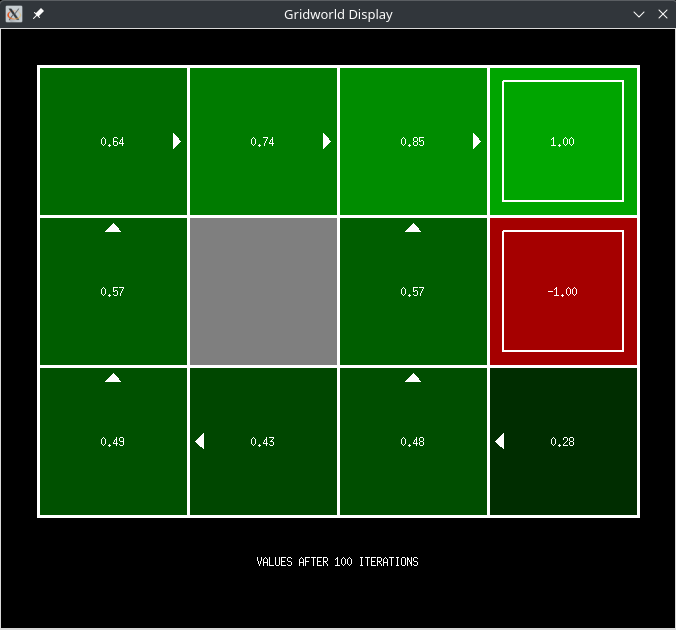
\includegraphics[width=0.5\textwidth]{./.img/ej11.png}
          \caption{Iteración de valores}
        \end{figure}
        python gridworld.py -a value -i 5
        \begin{figure}[H]
          \centering
          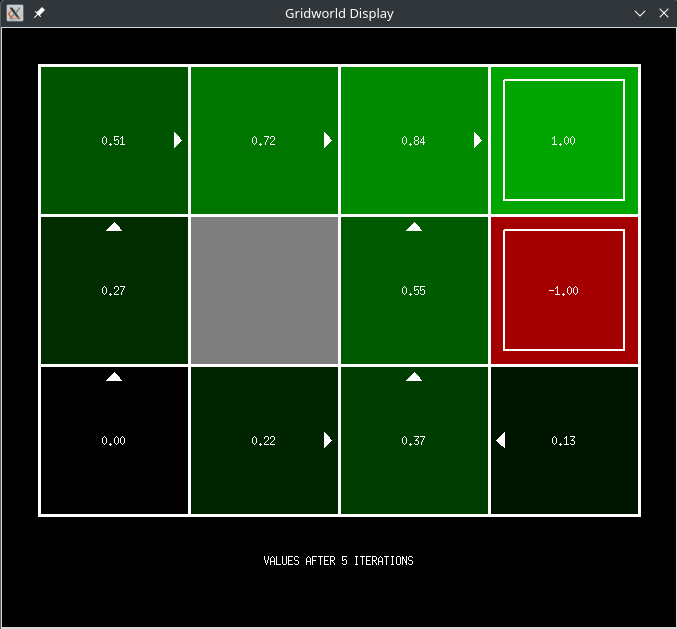
\includegraphics[width=0.5\textwidth]{./.img/ej12.png}
          \caption{Iteración de valores}
        \end{figure}
        \clearpage
      \subsection{Análisis de cruce de puentes} % * TERMINADO
        python gridworld.py -a value -i 100 -g BridgeGrid --discount 0.9 --noise 0.2
        \begin{figure}[H]
          \centering
          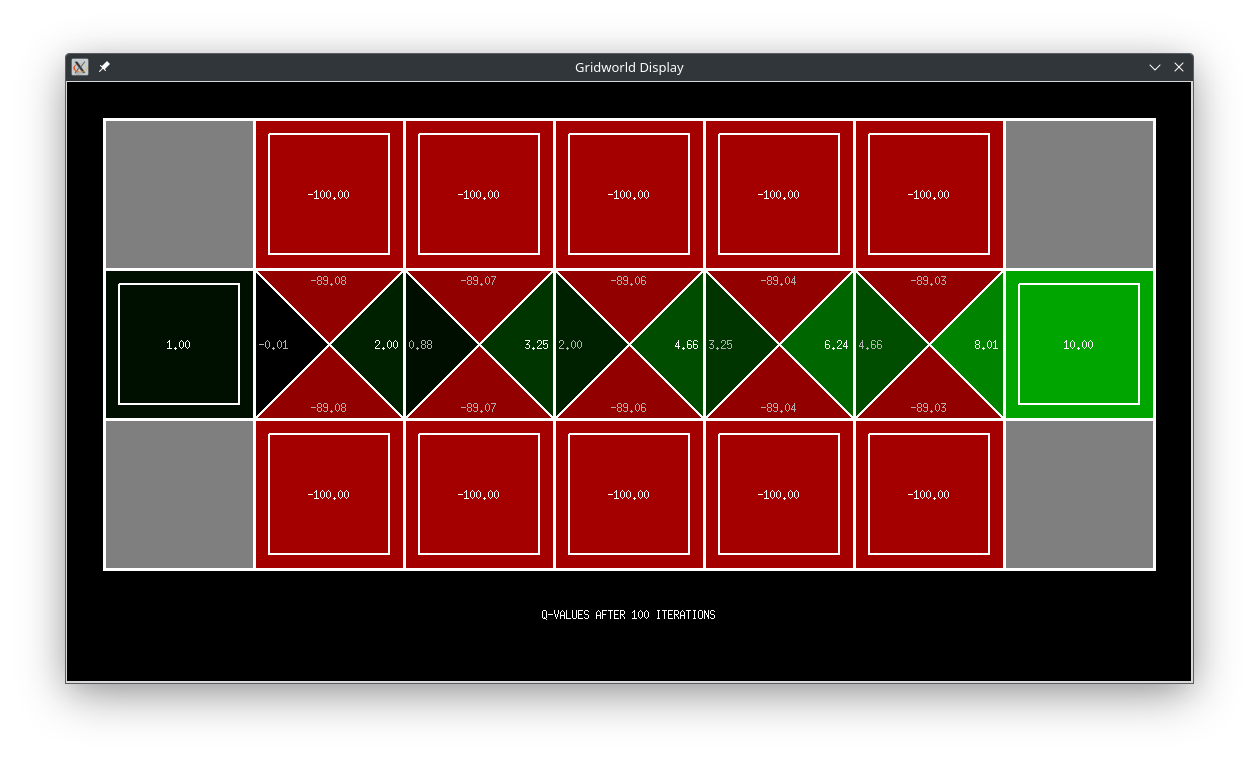
\includegraphics[width=0.8\textwidth]{./.img/ej21.png}
          \caption{Análisis de cruce de puentes}
        \end{figure}
        \clearpage
      \subsection{Q-Learning} % * TERMINADO
        python gridworld.py -aq -k 5 -m
        \begin{figure}[H]
          \centering
          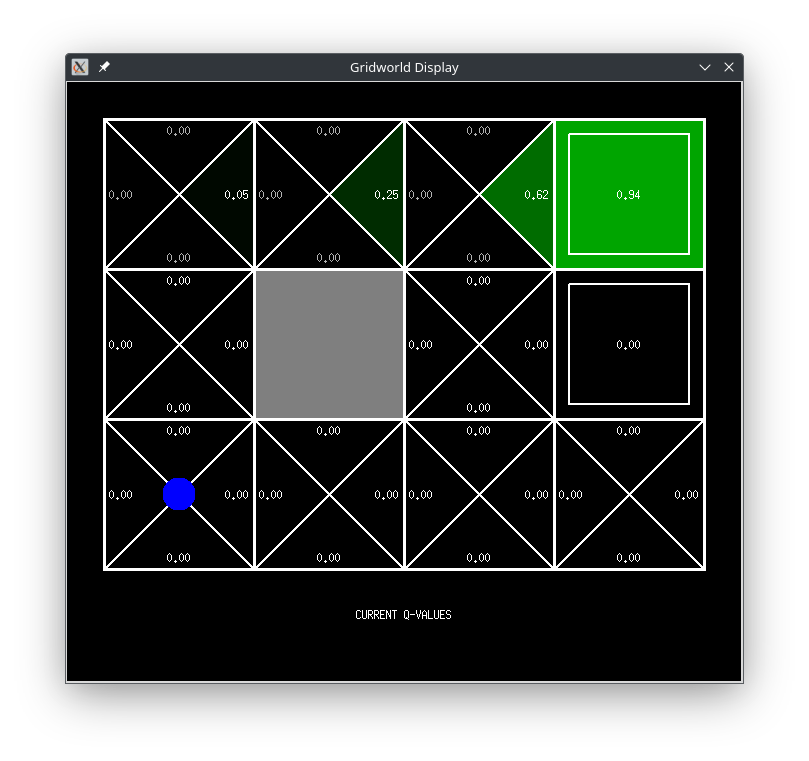
\includegraphics[width=0.8\textwidth]{./.img/ej31.png}
          \caption{Q-Learning}
        \end{figure}
        \clearpage
      \subsection{Epsilon Greedy} % * TERMINADO
        python gridworld.py -aq -k 100 - ruido 0.0 -e 0.1
        \begin{figure}[H]
          \centering
          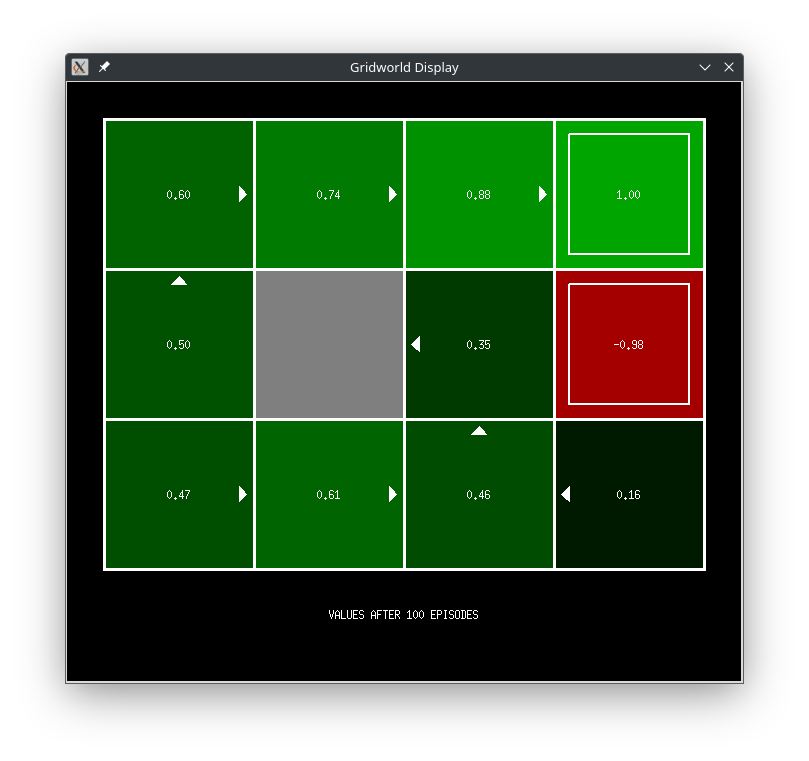
\includegraphics[width=0.55\textwidth]{./.img/ej41.png}
          \caption{Epsilon Greedy}
        \end{figure}
        python gridworld.py -aq -k 100 - ruido 0.0 -e 0.9
        \begin{figure}[H]
          \centering
          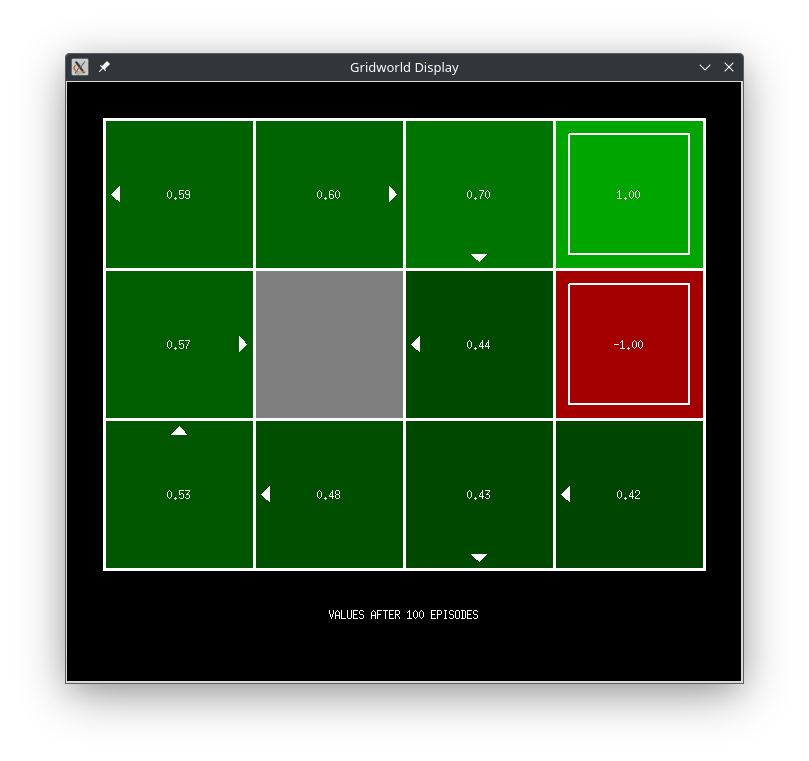
\includegraphics[width=0.55\textwidth]{./.img/ej42.png}
          \caption{Epsilon Greedy}
        \end{figure}
        \clearpage
      \subsection{Q-Learning y Pacman} % * TERMINADO
\begin{lstlisting}[language=Python, caption=Ejecución de Q-Learning y Pacman 1]
python pacman.py -p PacmanQAgent -x 2000 -n 2010 -l smallGrid
Beginning 2000 episodes of Training
Reinforcement Learning Status:
        Completed 100 out of 2000 training episodes
        Average Rewards over all training: -510.01
        Average Rewards for last 100 episodes: -510.01
        Episode took 0.32 seconds
Reinforcement Learning Status:
        Completed 200 out of 2000 training episodes
        Average Rewards over all training: -510.93
        Average Rewards for last 100 episodes: -511.84
        Episode took 0.52 seconds
Reinforcement Learning Status:
        Completed 300 out of 2000 training episodes
        Average Rewards over all training: -491.66
        Average Rewards for last 100 episodes: -453.12
        Episode took 0.65 seconds
Reinforcement Learning Status:
        Completed 400 out of 2000 training episodes
        Average Rewards over all training: -444.42
        Average Rewards for last 100 episodes: -302.71
        Episode took 0.69 seconds
Reinforcement Learning Status:
        Completed 500 out of 2000 training episodes
        Average Rewards over all training: -405.61
        Average Rewards for last 100 episodes: -250.38
        Episode took 0.71 seconds
Reinforcement Learning Status:
        Completed 600 out of 2000 training episodes
        Average Rewards over all training: -381.12
        Average Rewards for last 100 episodes: -258.65
        Episode took 0.68 seconds
Reinforcement Learning Status:
        Completed 700 out of 2000 training episodes
        Average Rewards over all training: -373.79
        Average Rewards for last 100 episodes: -329.83
        Episode took 0.67 seconds
Reinforcement Learning Status:
        Completed 800 out of 2000 training episodes
        Average Rewards over all training: -354.59
        Average Rewards for last 100 episodes: -220.17
        Episode took 0.71 seconds
Reinforcement Learning Status:
        Completed 900 out of 2000 training episodes
        Average Rewards over all training: -332.85
        Average Rewards for last 100 episodes: -158.96
        Episode took 0.78 seconds
Reinforcement Learning Status:
        Completed 1000 out of 2000 training episodes
        Average Rewards over all training: -308.47
        Average Rewards for last 100 episodes: -89.04
        Episode took 0.76 seconds
Reinforcement Learning Status:
        Completed 1100 out of 2000 training episodes
        Average Rewards over all training: -288.34
        Average Rewards for last 100 episodes: -86.98
        Episode took 0.70 seconds
Reinforcement Learning Status:
        Completed 1200 out of 2000 training episodes
        Average Rewards over all training: -262.40
        Average Rewards for last 100 episodes: 22.94
        Episode took 0.77 seconds
Reinforcement Learning Status:
        Completed 1300 out of 2000 training episodes
        Average Rewards over all training: -228.72
        Average Rewards for last 100 episodes: 175.45
        Episode took 0.74 seconds
Reinforcement Learning Status:
        Completed 1400 out of 2000 training episodes
        Average Rewards over all training: -199.15
        Average Rewards for last 100 episodes: 185.15
        Episode took 0.75 seconds
Reinforcement Learning Status:
        Completed 1500 out of 2000 training episodes
        Average Rewards over all training: -174.12
        Average Rewards for last 100 episodes: 176.33
        Episode took 0.72 seconds
Reinforcement Learning Status:
        Completed 1600 out of 2000 training episodes
        Average Rewards over all training: -152.28
        Average Rewards for last 100 episodes: 175.30
        Episode took 0.75 seconds
Reinforcement Learning Status:
        Completed 1700 out of 2000 training episodes
        Average Rewards over all training: -133.01
        Average Rewards for last 100 episodes: 175.43
        Episode took 0.81 seconds
Reinforcement Learning Status:
        Completed 1800 out of 2000 training episodes
        Average Rewards over all training: -117.50
        Average Rewards for last 100 episodes: 146.05
        Episode took 0.71 seconds
Reinforcement Learning Status:
        Completed 1900 out of 2000 training episodes
        Average Rewards over all training: -98.88
        Average Rewards for last 100 episodes: 236.37
        Episode took 0.74 seconds
Reinforcement Learning Status:
        Completed 2000 out of 2000 training episodes
        Average Rewards over all training: -87.15
        Average Rewards for last 100 episodes: 135.61
        Episode took 0.73 seconds
Training Done (turning off epsilon and alpha)
---------------------------------------------
Pacman emerges victorious! Score: 499
Pacman emerges victorious! Score: 503
Pacman emerges victorious! Score: 499
Pacman emerges victorious! Score: 499
Pacman emerges victorious! Score: 499
Pacman emerges victorious! Score: 503
Pacman emerges victorious! Score: 499
Pacman emerges victorious! Score: 499
Pacman emerges victorious! Score: 499
Pacman emerges victorious! Score: 499
Average Score: 499.8
Scores:        499.0, 503.0, 499.0, 499.0, 499.0, 503.0, 499.0, 499.0, 499.0, 499.0
Win Rate:      10/10 (1.00)
Record:        Win, Win, Win, Win, Win, Win, Win, Win, Win, Win
\end{lstlisting}
\begin{lstlisting}[language=Python, caption=Ejecución de Q-Learning y Pacman 2]
python pacman.py -p PacmanQAgent -n 10 -l smallGrid -a numTraining=10
Beginning 10 episodes of Training
Pacman died! Score: -507
Pacman died! Score: -507
Pacman died! Score: -508
Pacman died! Score: -505
Pacman died! Score: -518
Pacman died! Score: -507
Pacman died! Score: -508
Pacman died! Score: -510
Pacman died! Score: -515
Pacman died! Score: -506
Training Done (turning off epsilon and alpha)
---------------------------------------------
Average Score: -509.1
Scores:        -507.0, -507.0, -508.0, -505.0, -518.0, -507.0, -508.0, -510.0, -515.0, -506.0
Win Rate:      0/10 (0.00)
Record:        Loss, Loss, Loss, Loss, Loss, Loss, Loss, Loss, Loss, Loss
\end{lstlisting}
        \clearpage
      \subsection{Q-Learning aproximado} % * TERMINADO
\begin{lstlisting}[language=Python, caption=Q-Learning aproximado]
python pacman.py -p ApproximateQAgent -x 2000 -n 2010 -l smallGrid
Beginning 2000 episodes of Training
Reinforcement Learning Status:
        Completed 100 out of 2000 training episodes
        Average Rewards over all training: -509.14
        Average Rewards for last 100 episodes: -509.14
        Episode took 0.43 seconds
Reinforcement Learning Status:
        Completed 200 out of 2000 training episodes
        Average Rewards over all training: -495.69
        Average Rewards for last 100 episodes: -482.23
        Episode took 0.69 seconds
Reinforcement Learning Status:
        Completed 300 out of 2000 training episodes
        Average Rewards over all training: -457.67
        Average Rewards for last 100 episodes: -381.63
        Episode took 0.81 seconds
Reinforcement Learning Status:
        Completed 400 out of 2000 training episodes
        Average Rewards over all training: -445.92
        Average Rewards for last 100 episodes: -410.67
        Episode took 0.81 seconds
Reinforcement Learning Status:
        Completed 500 out of 2000 training episodes
        Average Rewards over all training: -418.67
        Average Rewards for last 100 episodes: -309.68
        Episode took 0.85 seconds
Reinforcement Learning Status:
        Completed 600 out of 2000 training episodes
        Average Rewards over all training: -395.56
        Average Rewards for last 100 episodes: -280.02
        Episode took 0.87 seconds
Reinforcement Learning Status:
        Completed 700 out of 2000 training episodes
        Average Rewards over all training: -380.61
        Average Rewards for last 100 episodes: -290.93
        Episode took 0.88 seconds
Reinforcement Learning Status:
        Completed 800 out of 2000 training episodes
        Average Rewards over all training: -351.85
        Average Rewards for last 100 episodes: -150.51
        Episode took 0.97 seconds
Reinforcement Learning Status:
        Completed 900 out of 2000 training episodes
        Average Rewards over all training: -331.76
        Average Rewards for last 100 episodes: -171.02
        Episode took 1.02 seconds
Reinforcement Learning Status:
        Completed 1000 out of 2000 training episodes
        Average Rewards over all training: -302.39
        Average Rewards for last 100 episodes: -38.04
        Episode took 0.95 seconds
Reinforcement Learning Status:
        Completed 1100 out of 2000 training episodes
        Average Rewards over all training: -277.31
        Average Rewards for last 100 episodes: -26.55
        Episode took 0.94 seconds
Reinforcement Learning Status:
        Completed 1200 out of 2000 training episodes
        Average Rewards over all training: -254.64
        Average Rewards for last 100 episodes: -5.31
        Episode took 0.93 seconds
Reinforcement Learning Status:
        Completed 1300 out of 2000 training episodes
        Average Rewards over all training: -221.53
        Average Rewards for last 100 episodes: 175.84
        Episode took 0.94 seconds
Reinforcement Learning Status:
        Completed 1400 out of 2000 training episodes
        Average Rewards over all training: -193.09
        Average Rewards for last 100 episodes: 176.57
        Episode took 0.92 seconds
Reinforcement Learning Status:
        Completed 1500 out of 2000 training episodes
        Average Rewards over all training: -165.84
        Average Rewards for last 100 episodes: 215.79
        Episode took 0.94 seconds
Reinforcement Learning Status:
        Completed 1600 out of 2000 training episodes
        Average Rewards over all training: -143.87
        Average Rewards for last 100 episodes: 185.66
        Episode took 0.96 seconds
Reinforcement Learning Status:
        Completed 1700 out of 2000 training episodes
        Average Rewards over all training: -117.95
        Average Rewards for last 100 episodes: 296.68
        Episode took 0.98 seconds
Reinforcement Learning Status:
        Completed 1800 out of 2000 training episodes
        Average Rewards over all training: -98.24
        Average Rewards for last 100 episodes: 236.87
        Episode took 0.91 seconds
Reinforcement Learning Status:
        Completed 1900 out of 2000 training episodes
        Average Rewards over all training: -82.76
        Average Rewards for last 100 episodes: 195.92
        Episode took 0.96 seconds
Reinforcement Learning Status:
        Completed 2000 out of 2000 training episodes
        Average Rewards over all training: -64.30
        Average Rewards for last 100 episodes: 286.37
        Episode took 0.97 seconds
Training Done (turning off epsilon and alpha)
---------------------------------------------
Pacman emerges victorious! Score: 499
Pacman emerges victorious! Score: 499
Pacman emerges victorious! Score: 502
Pacman emerges victorious! Score: 499
Pacman emerges victorious! Score: 502
Pacman emerges victorious! Score: 495
Pacman emerges victorious! Score: 495
Pacman emerges victorious! Score: 503
Pacman emerges victorious! Score: 495
Pacman emerges victorious! Score: 503
Average Score: 499.2
Scores:        499.0, 499.0, 502.0, 499.0, 502.0, 495.0, 495.0, 503.0, 495.0, 503.0
Win Rate:      10/10 (1.00)
Record:        Win, Win, Win, Win, Win, Win, Win, Win, Win, Win
\end{lstlisting}
\begin{lstlisting}[language=Python, caption=Q-Learning aproximado]
python pacman.py -p ApproximateQAgent -a extractor=SimpleExtractor -x 50 -n 60 -l mediumGrid      
Beginning 50 episodes of Training
Training Done (turning off epsilon and alpha)
---------------------------------------------
Pacman emerges victorious! Score: 525
Pacman emerges victorious! Score: 527
Pacman emerges victorious! Score: 521
Pacman emerges victorious! Score: 529
Pacman emerges victorious! Score: 529
Pacman emerges victorious! Score: 527
Pacman emerges victorious! Score: 529
Pacman emerges victorious! Score: 525
Pacman emerges victorious! Score: 529
Pacman emerges victorious! Score: 529
Average Score: 527.0
Scores:        525.0, 527.0, 521.0, 529.0, 529.0, 527.0, 529.0, 525.0, 529.0, 529.0
Win Rate:      10/10 (1.00)
Record:        Win, Win, Win, Win, Win, Win, Win, Win, Win, Win
\end{lstlisting}
\begin{lstlisting}[language=Python, caption=Q-Learning aproximado]
python pacman.py -p ApproximateQAgent -a extractor=SimpleExtractor -x 50 -n 60 -l mediumClassic
Beginning 50 episodes of Training
Training Done (turning off epsilon and alpha)
---------------------------------------------
Pacman emerges victorious! Score: 1330
Pacman emerges victorious! Score: 1337
Pacman emerges victorious! Score: 1335
Pacman emerges victorious! Score: 1329
Pacman emerges victorious! Score: 1332
Pacman died! Score: 68
Pacman emerges victorious! Score: 1324
Pacman emerges victorious! Score: 1322
Pacman emerges victorious! Score: 1336
Pacman emerges victorious! Score: 1329
Average Score: 1204.2
Scores:        1330.0, 1337.0, 1335.0, 1329.0, 1332.0, 68.0, 1324.0, 1322.0, 1336.0, 1329.0
Win Rate:      9/10 (0.90)
Record:        Win, Win, Win, Win, Win, Loss, Win, Win, Win, Win
\end{lstlisting}
    \cpsection{Autograder} % * TERMINADO
\begin{lstlisting}[language=Python, caption=Autograder]
python autograder.py
Starting on 12-17 at 17:23:30

Question q1
===========

*** PASS: test_cases/q1/1-tinygrid.test
*** PASS: test_cases/q1/2-tinygrid-noisy.test
*** PASS: test_cases/q1/3-bridge.test
*** PASS: test_cases/q1/4-discountgrid.test

### Question q1: 4/4 ###


Question q2
===========

*** PASS: test_cases/q2/1-bridge-grid.test

### Question q2: 1/1 ###


Question q3
===========

*** PASS: test_cases/q3/1-tinygrid.test
*** PASS: test_cases/q3/2-tinygrid-noisy.test
*** PASS: test_cases/q3/3-bridge.test
*** PASS: test_cases/q3/4-discountgrid.test

### Question q3: 4/4 ###


Question q4
===========

*** PASS: test_cases/q4/1-tinygrid.test
*** PASS: test_cases/q4/2-tinygrid-noisy.test
*** PASS: test_cases/q4/3-bridge.test
*** PASS: test_cases/q4/4-discountgrid.test

### Question q4: 2/2 ###


Question q5
===========

Beginning 2000 episodes of Training
Reinforcement Learning Status:
	Completed 100 out of 2000 training episodes
	Average Rewards over all training: -510.09
	Average Rewards for last 100 episodes: -510.09
	Episode took 0.32 seconds
Reinforcement Learning Status:
	Completed 200 out of 2000 training episodes
	Average Rewards over all training: -511.44
	Average Rewards for last 100 episodes: -512.78
	Episode took 0.52 seconds
Reinforcement Learning Status:
	Completed 300 out of 2000 training episodes
	Average Rewards over all training: -474.83
	Average Rewards for last 100 episodes: -401.61
	Episode took 0.58 seconds
Reinforcement Learning Status:
	Completed 400 out of 2000 training episodes
	Average Rewards over all training: -443.94
	Average Rewards for last 100 episodes: -351.28
	Episode took 0.66 seconds
Reinforcement Learning Status:
	Completed 500 out of 2000 training episodes
	Average Rewards over all training: -425.37
	Average Rewards for last 100 episodes: -351.08
	Episode took 0.69 seconds
Reinforcement Learning Status:
	Completed 600 out of 2000 training episodes
	Average Rewards over all training: -392.55
	Average Rewards for last 100 episodes: -228.44
	Episode took 0.66 seconds
Reinforcement Learning Status:
	Completed 700 out of 2000 training episodes
	Average Rewards over all training: -361.91
	Average Rewards for last 100 episodes: -178.11
	Episode took 0.68 seconds
Reinforcement Learning Status:
	Completed 800 out of 2000 training episodes
	Average Rewards over all training: -345.18
	Average Rewards for last 100 episodes: -228.07
	Episode took 0.66 seconds
Reinforcement Learning Status:
	Completed 900 out of 2000 training episodes
	Average Rewards over all training: -331.22
	Average Rewards for last 100 episodes: -219.49
	Episode took 0.76 seconds
Reinforcement Learning Status:
	Completed 1000 out of 2000 training episodes
	Average Rewards over all training: -312.16
	Average Rewards for last 100 episodes: -140.62
	Episode took 0.79 seconds
Reinforcement Learning Status:
	Completed 1100 out of 2000 training episodes
	Average Rewards over all training: -288.21
	Average Rewards for last 100 episodes: -48.77
	Episode took 0.79 seconds
Reinforcement Learning Status:
	Completed 1200 out of 2000 training episodes
	Average Rewards over all training: -270.74
	Average Rewards for last 100 episodes: -78.52
	Episode took 0.76 seconds
Reinforcement Learning Status:
	Completed 1300 out of 2000 training episodes
	Average Rewards over all training: -243.37
	Average Rewards for last 100 episodes: 85.10
	Episode took 0.71 seconds
Reinforcement Learning Status:
	Completed 1400 out of 2000 training episodes
	Average Rewards over all training: -220.66
	Average Rewards for last 100 episodes: 74.50
	Episode took 0.72 seconds
Reinforcement Learning Status:
	Completed 1500 out of 2000 training episodes
	Average Rewards over all training: -190.82
	Average Rewards for last 100 episodes: 226.94
	Episode took 0.69 seconds
Reinforcement Learning Status:
	Completed 1600 out of 2000 training episodes
	Average Rewards over all training: -161.59
	Average Rewards for last 100 episodes: 276.94
	Episode took 0.70 seconds
Reinforcement Learning Status:
	Completed 1700 out of 2000 training episodes
	Average Rewards over all training: -141.72
	Average Rewards for last 100 episodes: 176.13
	Episode took 0.70 seconds
Reinforcement Learning Status:
	Completed 1800 out of 2000 training episodes
	Average Rewards over all training: -121.80
	Average Rewards for last 100 episodes: 216.92
	Episode took 0.69 seconds
Reinforcement Learning Status:
	Completed 1900 out of 2000 training episodes
	Average Rewards over all training: -105.07
	Average Rewards for last 100 episodes: 195.96
	Episode took 0.76 seconds
Reinforcement Learning Status:
	Completed 2000 out of 2000 training episodes
	Average Rewards over all training: -89.46
	Average Rewards for last 100 episodes: 207.10
	Episode took 0.67 seconds
Training Done (turning off epsilon and alpha)
---------------------------------------------
Pacman emerges victorious! Score: 503
Pacman emerges victorious! Score: 503
Pacman emerges victorious! Score: 499
Pacman emerges victorious! Score: 499
Pacman emerges victorious! Score: 503
Pacman emerges victorious! Score: 503
Pacman emerges victorious! Score: 503
Pacman emerges victorious! Score: 503
Pacman emerges victorious! Score: 495
Pacman emerges victorious! Score: 503
Pacman emerges victorious! Score: 499
Pacman emerges victorious! Score: 503
Pacman emerges victorious! Score: 503
Pacman emerges victorious! Score: 503
Pacman emerges victorious! Score: 503
Pacman emerges victorious! Score: 503
Pacman emerges victorious! Score: 495
Pacman emerges victorious! Score: 503
Pacman emerges victorious! Score: 503
Pacman emerges victorious! Score: 503
Pacman emerges victorious! Score: 503
Pacman emerges victorious! Score: 503
Pacman emerges victorious! Score: 503
Pacman emerges victorious! Score: 503
Pacman emerges victorious! Score: 499
Pacman emerges victorious! Score: 495
Pacman emerges victorious! Score: 503
Pacman emerges victorious! Score: 503
Pacman emerges victorious! Score: 495
Pacman emerges victorious! Score: 495
Pacman emerges victorious! Score: 495
Pacman emerges victorious! Score: 499
Pacman emerges victorious! Score: 499
Pacman emerges victorious! Score: 503
Pacman emerges victorious! Score: 503
Pacman emerges victorious! Score: 503
Pacman emerges victorious! Score: 503
Pacman emerges victorious! Score: 495
Pacman emerges victorious! Score: 499
Pacman emerges victorious! Score: 503
Pacman emerges victorious! Score: 495
Pacman emerges victorious! Score: 499
Pacman emerges victorious! Score: 503
Pacman emerges victorious! Score: 503
Pacman emerges victorious! Score: 503
Pacman emerges victorious! Score: 503
Pacman emerges victorious! Score: 499
Pacman emerges victorious! Score: 503
Pacman emerges victorious! Score: 495
Pacman emerges victorious! Score: 503
Pacman emerges victorious! Score: 503
Pacman emerges victorious! Score: 503
Pacman emerges victorious! Score: 503
Pacman emerges victorious! Score: 499
Pacman emerges victorious! Score: 503
Pacman emerges victorious! Score: 499
Pacman emerges victorious! Score: 503
Pacman emerges victorious! Score: 503
Pacman emerges victorious! Score: 499
Pacman emerges victorious! Score: 503
Pacman emerges victorious! Score: 503
Pacman emerges victorious! Score: 503
Pacman emerges victorious! Score: 503
Pacman emerges victorious! Score: 503
Pacman emerges victorious! Score: 495
Pacman emerges victorious! Score: 499
Pacman emerges victorious! Score: 503
Pacman emerges victorious! Score: 495
Pacman emerges victorious! Score: 499
Pacman emerges victorious! Score: 495
Pacman emerges victorious! Score: 495
Pacman emerges victorious! Score: 503
Pacman emerges victorious! Score: 495
Pacman emerges victorious! Score: 503
Pacman emerges victorious! Score: 499
Pacman emerges victorious! Score: 503
Pacman emerges victorious! Score: 503
Pacman emerges victorious! Score: 503
Pacman emerges victorious! Score: 495
Pacman emerges victorious! Score: 495
Pacman emerges victorious! Score: 503
Pacman emerges victorious! Score: 503
Pacman emerges victorious! Score: 499
Pacman emerges victorious! Score: 503
Pacman emerges victorious! Score: 503
Pacman emerges victorious! Score: 495
Pacman emerges victorious! Score: 499
Pacman emerges victorious! Score: 503
Pacman emerges victorious! Score: 503
Pacman emerges victorious! Score: 503
Pacman emerges victorious! Score: 499
Pacman emerges victorious! Score: 503
Pacman emerges victorious! Score: 503
Pacman emerges victorious! Score: 503
Pacman emerges victorious! Score: 499
Pacman emerges victorious! Score: 499
Pacman emerges victorious! Score: 495
Pacman emerges victorious! Score: 499
Pacman emerges victorious! Score: 499
Pacman emerges victorious! Score: 503
Reinforcement Learning Status:
	Completed 100 test episodes
	Average Rewards over testing: 500.68
	Average Rewards for last 100 episodes: 500.68
	Episode took 0.67 seconds
Average Score: 500.68
Scores:        503.0, 503.0, 499.0, 499.0, 503.0, 503.0, 503.0, 503.0, 495.0, 503.0, 499.0, 503.0, 503.0, 503.0, 503.0, 503.0, 495.0, 503.0, 503.0, 503.0, 503.0, 503.0, 503.0, 503.0, 499.0, 495.0, 503.0, 503.0, 495.0, 495.0, 495.0, 499.0, 499.0, 503.0, 503.0, 503.0, 503.0, 495.0, 499.0, 503.0, 495.0, 499.0, 503.0, 503.0, 503.0, 503.0, 499.0, 503.0, 495.0, 503.0, 503.0, 503.0, 503.0, 499.0, 503.0, 499.0, 503.0, 503.0, 499.0, 503.0, 503.0, 503.0, 503.0, 503.0, 495.0, 499.0, 503.0, 495.0, 499.0, 495.0, 495.0, 503.0, 495.0, 503.0, 499.0, 503.0, 503.0, 503.0, 495.0, 495.0, 503.0, 503.0, 499.0, 503.0, 503.0, 495.0, 499.0, 503.0, 503.0, 503.0, 499.0, 503.0, 503.0, 503.0, 499.0, 499.0, 495.0, 499.0, 499.0, 503.0
Win Rate:      100/100 (1.00)
Record:        Win, Win, Win, Win, Win, Win, Win, Win, Win, Win, Win, Win, Win, Win, Win, Win, Win, Win, Win, Win, Win, Win, Win, Win, Win, Win, Win, Win, Win, Win, Win, Win, Win, Win, Win, Win, Win, Win, Win, Win, Win, Win, Win, Win, Win, Win, Win, Win, Win, Win, Win, Win, Win, Win, Win, Win, Win, Win, Win, Win, Win, Win, Win, Win, Win, Win, Win, Win, Win, Win, Win, Win, Win, Win, Win, Win, Win, Win, Win, Win, Win, Win, Win, Win, Win, Win, Win, Win, Win, Win, Win, Win, Win, Win, Win, Win, Win, Win, Win, Win
*** PASS: test_cases/q5/grade-agent.test (1 of 1 points)
***     Grading agent using command:  python pacman.py -p PacmanQAgent -x 2000 -n 2100 -l smallGrid -q -f --fixRandomSeed
***     100 wins (1 of 1 points)
***         Grading scheme:
***          < 70:  0 points
***         >= 70:  1 points

### Question q5: 1/1 ###


Question q6
===========

*** PASS: test_cases/q6/1-tinygrid.test
*** PASS: test_cases/q6/2-tinygrid-noisy.test
*** PASS: test_cases/q6/3-bridge.test
*** PASS: test_cases/q6/4-discountgrid.test
*** PASS: test_cases/q6/5-coord-extractor.test

### Question q6: 3/3 ###


Finished at 17:23:45

Provisional grades
==================
Question q1: 4/4
Question q2: 1/1
Question q3: 4/4
Question q4: 2/2
Question q5: 1/1
Question q6: 3/3
------------------
Total: 15/15

Your grades are NOT yet registered.  To register your grades, make sure
to follow your instructor's guidelines to receive credit on your project.


\end{lstlisting}
\end{document}